% -------------------------------------------------------------
% IMPLEMENTATION AND TECHNICAL REALIZATION
% -------------------------------------------------------------


\noindent HeatItOn is divided into three sections, and two versions. First there is the midterm evaluation demo version, and then there is the final version. We will go through both to see the first implementation and the improvements and changes that we made for the final version. 

\section{Frontend Implementation}

\hspace*{1cm}Our Frontend Implementation is desgined with the plant operators in mind, keeping it simple and user friendly. To achieve this, we started with a UI-sketch where we tried to come up with an easy to use and easy to understand concept, that we tried to achieve in our implementation.
 	
The application is split into three different tabs. The first one, that the user sees when they launch the application is the Assets tab. Here the user can manage and see all the existing assets \cite{projectassetsdata}, they can import or export assets as csv's or manually add/remove or edit specific assets one by one. This page also has three preset toggles(Scenario 1, Scenario 2 and Custom). As the Assets page is where the operator will start the optimization process, by selecting the asset combination they want to optimize with, the toggles merely select from the assets the ones that are in that scenario. If they wish to optimize for a new scenario, they can select the Custom toggle, allowing them to run the optimization process for any scenario. After selecting the desired assets the user has to click on the Optimize button that will start the optimization process for the selected assets. 
	
The list of assets is connected through the backend with the database, each modification being done live in the database. The optimization process from the backend is called from the frontend by clicking a button. The Assets tab will send the Optimization algorithm the assets selected to be optimized every time the button is clicked.
	
The second tab, the Results tab is where, once the user started an optimization, the result of that run will appear. On the left side, they can see and select out of a list of all results. When they select one result, the user can see the hourly result in a table format or view the data in different graphs. They can also export them into csv's. If the user would like to focus on a specific time period, not the entire optimiziation run, they can use a date-time picker to select from when to until when they want to see the result data, which will affect the result table and the graphs as well.
	
The tab loads all the optimization-results from the database using the backend services.
	
The third tab, Sources, is where the user will upload/export or even edit source data. On the left, you can see a list of uploaded csv's again. When the user selects one, they can also visualize the source data in a few simple charts or see the entire source data in a table. The cells of the table are modifiable so they can also edit the source data.
	
This tab uploads all sources directly to the database, using the backend services, while the csv file's are handled locally.
	
Our goal with each tab was acheaving an easily navigable and understandable UI, while giving all the necessary tools for the plant-operators/users for adequate management. Although we only received source data for four weeks and two asset scenarios, we tried to create a scalable, modular UI, that can handle dozens of assets and years worth of source data. As a side goal we also wanted to achieve a simple yet modern and visually appealing look.

\subsection{Midterm Version}

\hspace*{1cm}For the midterm demo, we prioritised usability over aspect. As this version was a mere proof of concept, and its goal was to plant a picture of our way of implementing it and to show what we think is possible, some aspects of the overall user experience was ignored so we can focus on actual functionality.

This means that the UI for this version has a very generic, template look. Buttons are rough and placed where we could fit them, while icons are uninteresting and unintuitive. A majorly different approach for displaying assets, results and sources was used in this version. Instead of the frontend lists updating to changes accordingly(like uploading csv's or generating results) in real time, we added a refresh button that, when clicked, reloads all the data from the database. This solution was a compromise made for this version, and eliminating it, a focuspoint for the final version.

The Assets tab was fully functional, and only needed some visual and aesthetic improvements (see Appendix \ref{appendix:figures}).



The Results tab in this version is defined by minimalistic graphs, that made it hard to visualize the results. Our three graphs(electricity use/production, heat production and CO2 production) were a good start but we realised we need a lot more for proper visualization. (see Appendix \ref{appendix:figures}).

The Sources tab functioned as expected but the possibility to edit the csv data was missing from this version.

Overall the demo was a very solid proof of concept that helped us learn what we were missing for the final version while also showing us the direction we are going.
	
\subsection{Final Version}
\hspace*{1cm}The final version focuses more on user experience with minor fuctionality improvementse when compared to the midterm implementation. The primary goal of this version was to improve usability, visual appearance, and introduce additional statistical aspects while maintaining a consistent and scalable structure. 

A significant improvement is the change from a manual data refresh system to a dynamic, responsive interface. In contrast to the midterm version, where a dedicated refresh button was required to update data, the final implementation ensures that all lists and views update automatically in response to changes in the database. This enhancement improves workflow efficiency and eliminates unnecessary user interaction.

The visual design of the interface has been improved. The final version adopts a modern, structured design with consistent colors, clearer text formating, and improved spacing. Asset cards have been redesigned to display key information in a meaningful and readable format, including maximum heat, production cost, CO\textsubscript{2} emissions, and electricity generation/consumption. Additionally, asset categories such as gas, oil, electric, and motor are visually distinguished through icons and labels, allowing for faster recognition and comparison.

The scenario selection system has been refined and better integrated into the workflow. Instead of simple toggles, the final version introduces clearly defined scenario panels with descriptive labels such as “Peak Load,” “Eco Mode,” and “Custom Configure.” Each scenario communicates its purpose more effectively, enabling more intuitive decision-making. Furthermore, visual indicators highlight selected assets within each scenario, improving clarity during configuration.

Additional controls have been add, including a “Manager” and an “Optimize” button. The Manager section serves as a centralized interface for creating, importing, and exporting assets. These improvements lead to a clearer workflow, guiding the user from setup to execution in a more structured way.

The Results tab has undergone major enhancements in both data presentation and analytical depth. A summary dashboard has been introduced at the top of the page, presenting key performance indicators such as total heat production, net electricity balance, total CO\textsubscript{2} emissions, and total production cost. These aggregated metrics provide immediate insight into optimization outcomes without requiring detailed inspection of raw data.

The data display has also been improved with better formatting, clearer column labeling, and pagination support for large datasets. The addition of pagination ensures that even large datasets remain readable and manageable.

The charting system represents one of the most significant functional improvements. While the midterm version included only basic visualizations, the final version introduces a comprehensive set of charts:
\begin{itemize}
\item A stacked area chart showing heat production per asset over time, including a total heat overlay
\item A production cost per hour chart, allowing detailed financial analysis
\item A generator share pie chart, illustrating the contribution of each asset within a selected time range
\item An electricity usage and generation chart, displaying hourly electricity balance in MWh
\end{itemize}

These visualizations provide a deeper understanding of system behavior and allow users to analyze performance trends, cost distribution, and resource utilization more effectively. Interactivity elements, such as tooltips and time-range filtering, further enhance data exploration.
The date and time filtering functionality has been refined, with a more structured input system for selecting precise time intervals. Filtering affects both tabular and graphical outputs, ensuring consistency across all displayed data.

The Sources tab has also been expanded with important new functionality. Unlike the midterm version, the final implementation allows direct editing of source data within the table. This feature enables on-the-fly adjustments without requiring external file modification. The table design has been improved for clarity, and pagination has been introduced to handle large datasets efficiently.
File management capabilities have been enhanced, including clearer separation between uploaded files and active data views. Import and export functions remain available but are now better integrated into the interface.

Overall, the final version achieves a significantly higher level of usability, clarity, and analytical capability. The transition from a proof-of-concept interface to a polished, production-oriented design is evident across all tabs. The system now provides a comprehensive toolset for asset management, optimization execution, and result analysis, while maintaining a scalable and user-centered design approach.

\section{Backend Implementation}
\subsection{Midterm Version}

\hspace*{1cm}The backend is implemented using ASP.NET Core 9.0 and follows a layered architectural design that emphasizes modularity, scalability, and separation of concerns. The structure consists of Controllers, Services, Interfaces, Models, and a Data layer, each responsible for a distinct part of the system functionality.


\textbf{Architecture and Main Components}

\begin{figure}[H]
\centering
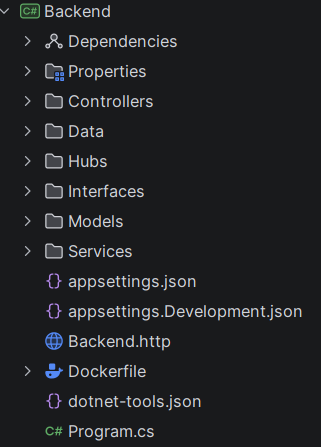
\includegraphics[width=0.6\textwidth]{Images/backend-file-structure.png}
\caption{Backend file structure showing the organization of controllers, services, interfaces, models, and data components.}
\label{fig:backend-structure}
\end{figure}

The backend is organized into clearly defined layers:

\begin{itemize}
    \item \textbf{Controllers}: Provide RESTful API endpoints and act as the entry point for client requests. Controllers are responsible for handling HTTP requests, binding input parameters, and returning appropriate responses.
    
    \item \textbf{Services}: Implement the core business logic. Each service corresponds to a domain entity, such as assets, source data, and optimization results. Services coordinate data processing and communicate with the persistence layer.
    
    \item \textbf{Models}: Represent domain entities and map directly to database tables. Examples include \texttt{Asset}, \texttt{Source}, \texttt{Result}, \texttt{ResultList}, and \texttt{OptimizedResults}.
    
    \item \textbf{Data Layer}: Contains the Entity Framework database context (\texttt{BackendDbContext}) and migration files. This layer manages communication with the MySQL database.
\end{itemize}

This architecture ensures that responsibilities are clearly separated, enabling easier maintenance and extensibility.


\textbf{API and Controller Design}

During the midterm the backend exposed basic REST endpoints (CRUD) implemented ad-hoc, these were formalized in the final version through generic controller/service interfaces (see the \textbf{Final Version} subsection).

All controller actions are implemented asynchronously using \texttt{Task<IActionResult>}, allowing efficient handling of concurrent requests. Controllers delegate processing tasks to the service layer, keeping the API layer thin and focused on HTTP concerns.


\textbf{Business Logic Handling}

All business logic is implemented within the service layer, which acts as the core processing unit of the backend. Each service implements the generic \texttt{IService<T>} interface, providing consistent operations across all entities.

Specialized services, such as the \texttt{OptimizerService}, encapsulate domain-specific logic related to heat production optimization. This includes processing input data, calculating results, and coordinating interactions between assets, source data, and result data.

The separation of business logic from controllers improves maintainability and enables independent testing of core functionality.


\textbf{Data Processing and Validation}

Data processing is primarily handled within the service layer. Incoming data from API requests is validated before being persisted or processed further. Validation mechanisms include:

\begin{itemize}
    \item Strongly typed C\# models for structured data representation
    \item Parameter binding and validation features provided by ASP.NET Core
    \item Logical validation rules implemented within service methods
\end{itemize}

This approach ensures that invalid or inconsistent data is prevented from entering the system and maintains overall data integrity.


\textbf{Database Communication}

The backend communicates with the MySQL database using Entity Framework. The \texttt{BackendDbContext} manages entity tracking, query execution, and persistence.

\begin{itemize}
    \item Models are mapped directly to database tables
    \item LINQ is used for querying and manipulating data
    \item Asynchronous database operations improve performance and scalability
\end{itemize}

Services interact with the database context to perform all data operations, ensuring controlled access to the persistence layer and preventing direct database access from controllers.


\textbf{System Behavior Support}

The backend supports the required system behavior by coordinating interactions between different system modules. Controllers expose endpoints for managing assets, source data, and optimization results, while services execute the corresponding logic.

The inclusion of a dedicated optimization service enables the processing of time-series data for heat demand and electricity prices, supporting the generation of optimized production schedules.


\textbf{Deployment Considerations}

The backend is deployed using Docker, which provides a consistent and isolated runtime environment. Containerization ensures that dependencies, configurations, and runtime settings are standardized across development and production environments.

This approach improves portability, simplifies deployment, and enhances the reliability of the backend infrastructure.


Overall, the backend implementation follows best practices for modern web application development, emphasizing modularity, scalability, and maintainability. The layered architecture ensures that the system can effectively support the required functionality while remaining adaptable to future enhancements.

\subsection{Final Version}
\hspace*{1cm}The final backend version extends the original layered ASP.NET Core architecture with additional runtime functionality and tighter system integration. We introduced two supporting components: a centralized exception-handling middleware and interface-based service contracts that define abstraction boundaries between controllers and services.

These additions work together with the existing layers as follows: controllers accept HTTP requests and delegate work to services; services implement business logic and interact with the data layer (EF `BackendDbContext`); both controllers and services rely on the `Interfaces` abstraction and dependency injection; the `ExceptionHandlingMiddleware` sits early in the request pipeline, catching exceptions from controllers and services, logging them, mapping domain errors to HTTP status codes, and returning compact JSON error responses. As a result, many local try/catch blocks were removed and method implementations became easily readable.

\begin{itemize}
    \item \textbf{Exception handling}: Centralized in \texttt{ExceptionHandlingMiddleware}. It intercepts exceptions thrown by controllers and services, logs them, maps domain errors to appropriate HTTP status codes, and returns a compact JSON payload (for example \texttt{\{}\texttt{"error":} \texttt{"<message>",}\texttt{"stackTrace":}\texttt{"<stackTrace>"}\texttt{\}}) with \texttt{Content-Type:}\texttt{application/json}. This provides consistent, machine-readable error responses for clients and prevents raw error details from leaking.
    \item \textbf{Interfaces}: Provide clear abstraction boundaries for controllers and services \\ (e.g., \texttt{IController <TCreate,TUpdate>}, \texttt{IService<T>}). Using interfaces enables dependency injection, easier unit testing, and consistent error-typing so the middleware can map domain exceptions to appropriate HTTP responses.
    \begin{itemize}
        \item The generic controller interface formalizes standard CRUD operations used across controllers:
        \begin{itemize}
            \item \texttt{List()} for retrieving collections of entities
            \item \texttt{Get(int id)} for retrieving a single entity
            \item \texttt{Post(TCreate model)} for creating new entries
            \item \texttt{Put(int id, TUpdate model)} for updating existing entries
            \item \texttt{Delete(int id)} for removing entries
        \end{itemize}
    \end{itemize}
    \item \textbf{Controllers}: Handle request/response concerns and remain thin — delegating business rules to services and relying on interfaces for testability, validate inputs.
    \item \textbf{Services}: Contain core business logic, interact with the data layer, and throw well-defined domain exceptions when needed. They do not implement HTTP concerns or repeated try/catch logic anymore.
    \item \textbf{Data layer}: The Entity Framework \texttt{BackendDbContext} and related repositories/models remain responsible for persistence and are used by services through interface-driven abstractions.
\end{itemize}

\section{Data Management}
\subsection{Midterm Version}
Data management is implemented using a relational database approach supported by MySQL, combined with an object-relational mapping layer provided by Entity Framework.

\textbf{Data Structure}

\begin{figure}[H]
\centering
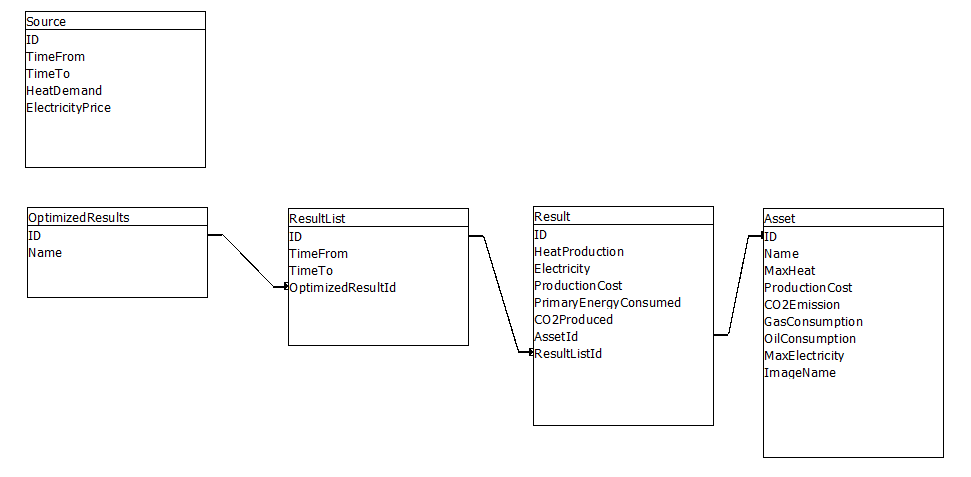
\includegraphics[width=1\textwidth]{Images/db-relations.png}
\caption{Database schema illustrating the relationships between Source, OptimizedResults, ResultList, Result, and Asset tables.}
\label{fig:db-schema}
\end{figure}

The data model is organized into five primary tables: Source, OptimizedResults, ResultList, Result, and Asset, each representing a distinct aspect of the system domain.
\begin{itemize}
\item The Source table stores time-based input data, including HeatDemand, and ElectricityPrice. This structure supports time-series data used for optimization processes.
\item The OptimizedResults table represents a container for optimization runs during the selected time period. 
\item The ResultList table links individual time intervals to a specific optimization result through the foreign key OptimizedResultId. Each entry contains results for separate assets within an hourly time frame, with attributes such as TimeFrom and TimeTo defining the interval. 
\item The Result table contains detailed output data generated by the optimization process. Attributes include HeatProduction, Electricity, ProductionCost, PrimaryEnergyConsumed, and CO2Produced. This table also includes foreign keys AssetId and ResultListId, establishing relationships with both Asset and ResultList. It stores the specific performance metrics for one asset in one hour.
\item The Asset table defines the characteristics of generators or boilers, including MaxHeat, ProductionCost, CO2Emission, GasConsumption, OilConsumption, MaxElectricity, and ImageName.
\end{itemize}

The relationships between these tables follow a hierarchical structure:
\begin{itemize}
\item One OptimizedResults entity relates to multiple ResultList entries.
\item One ResultList entry relates to multiple Result records.
\item Each Result references a single Asset.
\end{itemize}

Primary keys and foreign keys ensure referential integrity across all tables. For example, Result.AssetId must correspond to a valid entry in the Asset table, and ResultList.OptimizedResultId must reference an existing optimization result.

\textbf{Integration with Backend}

The data structure integrates directly with the backend through Entity Framework. Each database table is mapped to a corresponding C\# model, enabling seamless interaction between the application logic and the database layer. Entity Framework provides abstraction over raw SQL queries, allowing developers to interact with the database using LINQ queries and strongly typed objects. The DbContext component manages database connections, entity tracking, and query execution, ensuring consistent data access patterns across the application. Migration tools within Entity Framework support schema evolution, allowing controlled updates to the database structure while maintaining data integrity.

\textbf{Data Management Environment}

The database is deployed using Docker, ensuring a consistent and reproducible environment. The use of Docker also facilitates easy deployment, testing, and version control of the data management infrastructure.

Overall, the data management approach combines a well-defined relational schema, validation mechanisms, and seamless backend integration to ensure reliability, scalability, and maintainability of the system.

\subsection{Final Version}

\hspace*{1cm}The recent database updates were minor and mainly aimed at improving data quality. We added and refined several model-level validation rules using data-annotation attributes (such as Required, Range, and MaxLength) to prevent invalid or inconsistent values from being saved. We also introduced a unique constraint for the Source entity in the DbContext configuration to avoid creating duplicate entries. These changes strengthen validation and consistency across the system without altering the overall database structure.
